
% v2-acmsmall-sample.tex, dated March 6 2012
% This is a sample file for ACM small trim journals
%
% Compilation using 'acmsmall.cls' - version 1.3 (March 2012), Aptara Inc.
% (c) 2010 Association for Computing Machinery (ACM)
%
% Questions/Suggestions/Feedback should be addressed to => "acmtexsupport@aptaracorp.com".
% Users can also go through the FAQs available on the journal's submission webpage.
%
% Steps to compile: latex, bibtex, latex latex
%
% For tracking purposes => this is v1.3 - March 2012
\documentclass[prodmode,acmtecs]{acmsmall} % Aptara syntax
\usepackage[spanish,polish]{babel}
\usepackage[T1]{fontenc}
\usepackage{fancyvrb}
\usepackage{graphicx,hyperref}
\newcommand\cutout[1]{}


\usepackage[table]{xcolor}
\usepackage[utf8]{inputenc}
\usepackage[parfill]{parskip}
\usepackage{tabulary}
\PassOptionsToPackage{hyphens}{url}
\usepackage{hyperref}    
\usepackage[capitalize]{cleveref}


% Metadata Information
% !!! TODO: SET THESE VALUES !!!
\acmVolume{0}
\acmNumber{0}
\acmArticle{CFP}
\acmYear{0}
\acmMonth{0}

\newcounter{colstart}
\setcounter{page}{4}

\RecustomVerbatimCommand{\VerbatimInput}{VerbatimInput}%
{
%fontsize=\footnotesize,
fontfamily=\rmdefault
}


\newcommand{\UnderscoreCommands}{%\do\verbatiminput%
\do\citeNP \do\citeA \do\citeANP \do\citeN \do\shortcite%
\do\shortciteNP \do\shortciteA \do\shortciteANP \do\shortciteN%
\do\citeyear \do\citeyearNP%
}

\usepackage[strings]{underscore}



% Document starts
\begin{document}


\setcounter{colstart}{\thepage}

\acmArticle{CFP}
\title{{\huge\sc SIGLOG Monthly 238}

 June 2023}
\author{DAVID PURSER\affil{University of Liverpool, UK}
\vspace*{-2.6cm}\begin{flushright}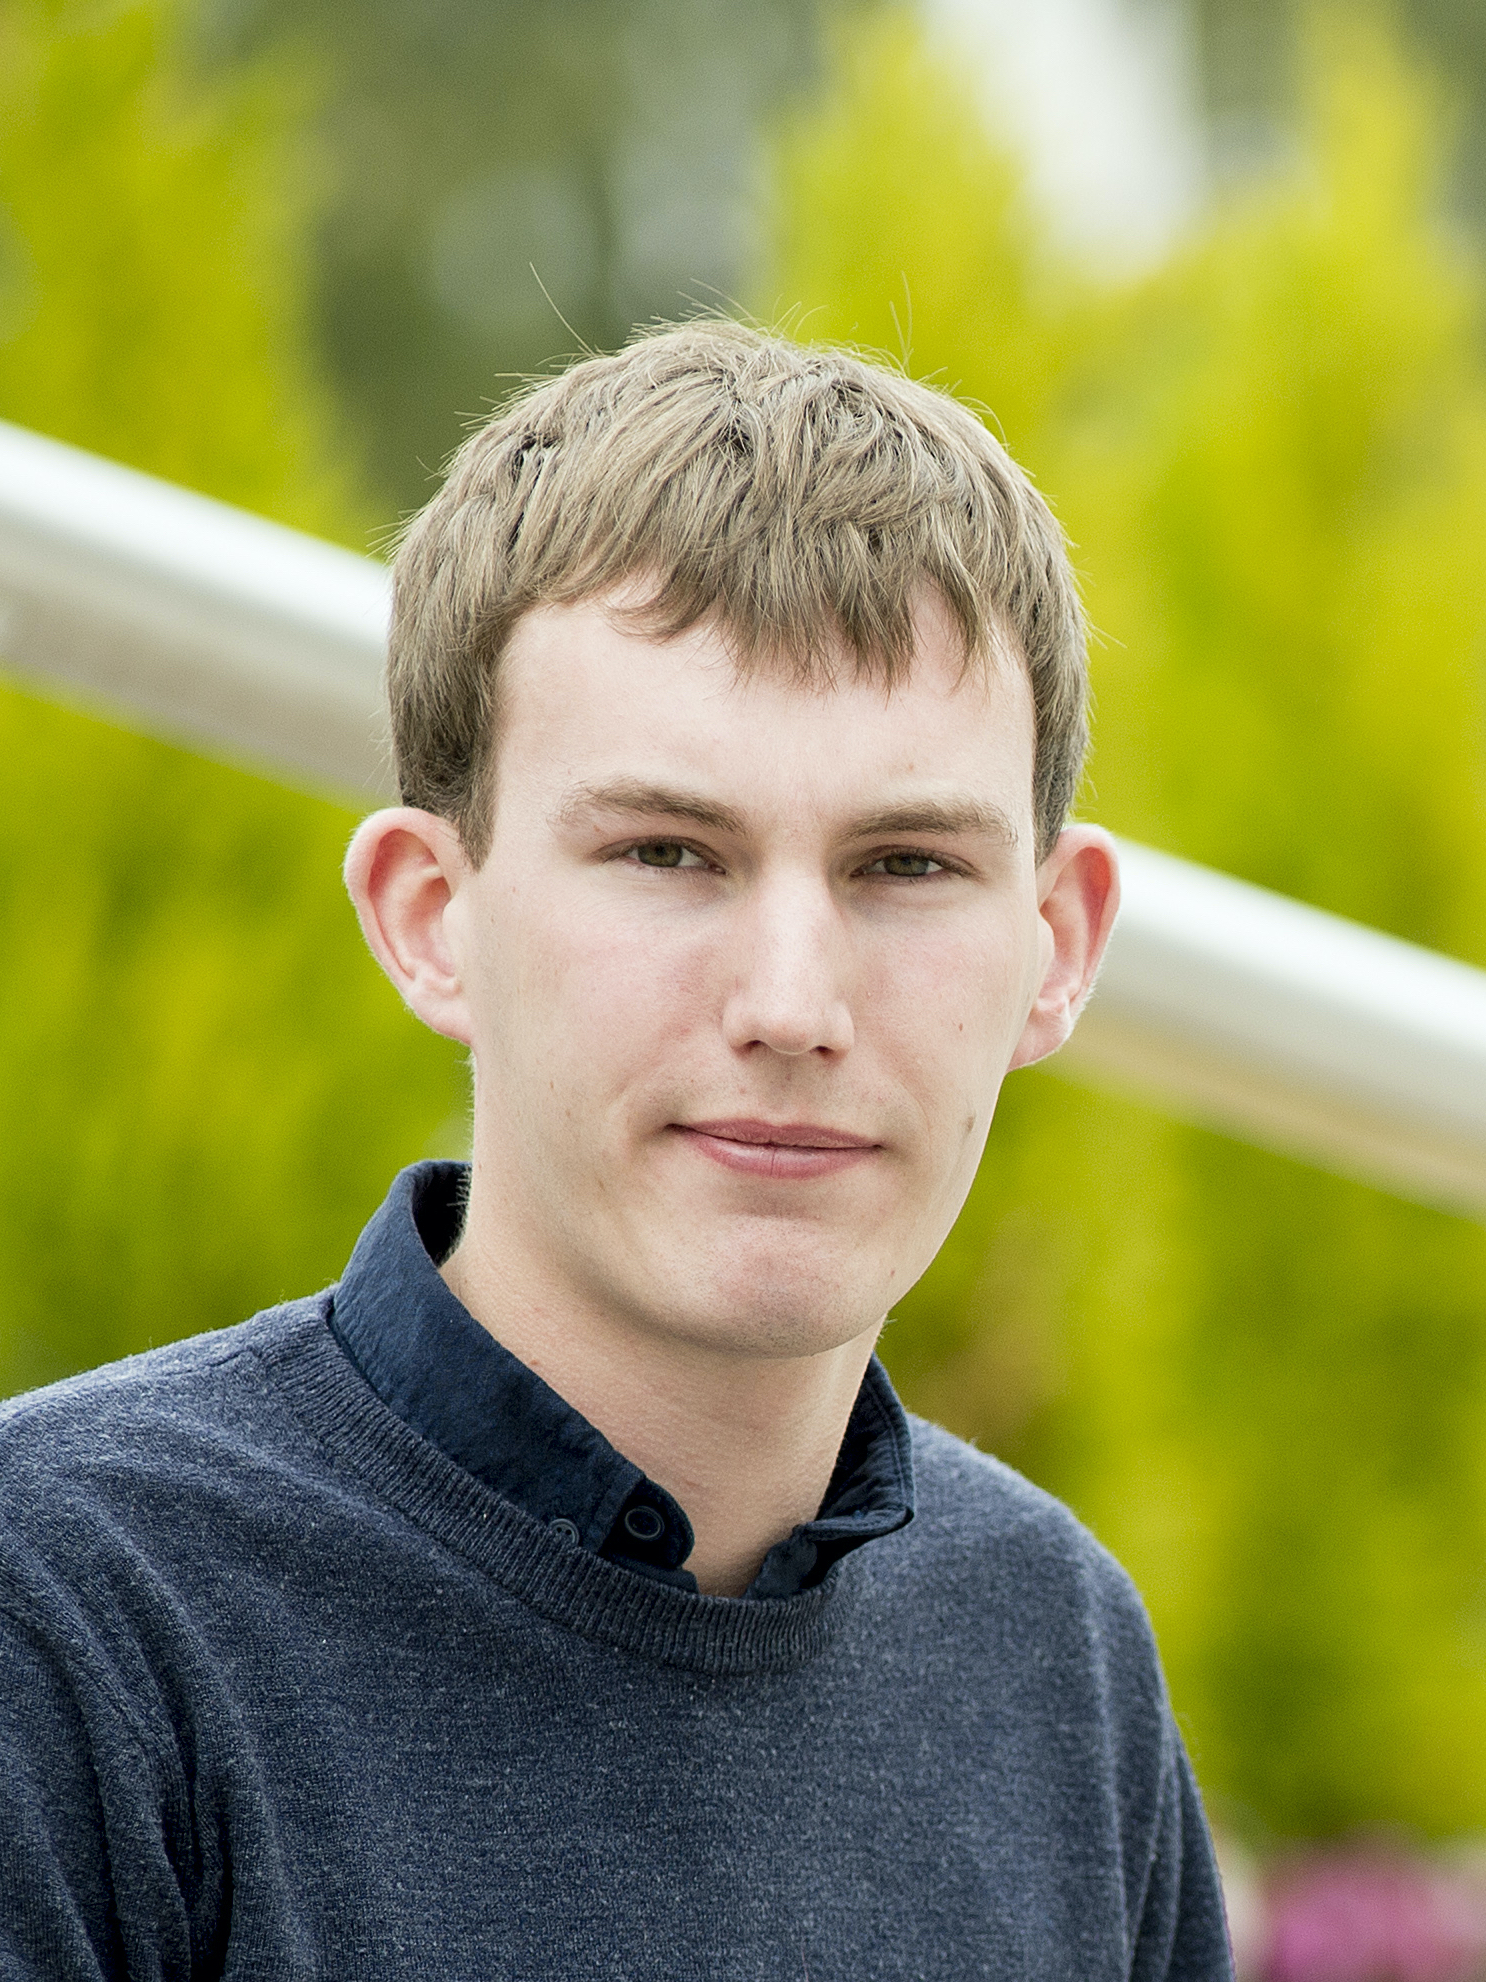
\includegraphics[width=30mm]{dp}\end{flushright}
}

\begin{abstract}
June 2023 edition of SIGLOG Monthly, featuring deadlines, calls and community announcements.
\end{abstract}


\maketitlee

\href{https://lics.siglog.org/newsletters/}{Past Issues}
 - 
\href{https://lics.siglog.org/newsletters/inst.html}{How to submit an announcement}
\section{Table of Content}\begin{itemize}\item DEADLINES (\cref{deadlines}) 
 
\item SIGLOG MATTERS 
 
\begin{itemize}\item Winner of the 2023 Alonzo Church Award (\cref{Winnerofthe2023AlonzoChurchAward})
\end{itemize} 
\item CALLS 
 
\begin{itemize}\item IWCS 2023 (CALL FOR PARTICIPATION) (\cref{IWCS2023})
\item CiE 2023 (CALL FOR PARTICIPATION, CALL FOR INFORMAL PRESENTATIONS) (\cref{CiE2023})
\item PhD Symposium iFM 2023 (CALL FOR PAPERS) (\cref{PhDSymposiumiFM2023})
\item ICALP 2023 (CALL FOR PARTICIPATION) (\cref{ICALP2023})
\item FSCD 2023 (CALL FOR PARTICIPATION) (\cref{FSCD2023})
\item CSL'24 (CALL FOR PAPERS) (\cref{CSL24})
\item RW 2023 (CALL FOR APPLICATIONS) (\cref{RW2023})
\end{itemize} 
\item JOB ANNOUNCEMENTS 
 
\begin{itemize}\item PhD and Post-doctoral Positions Available in Formal Methods for Reversible Concurrent Calculi Augusta University (Georgia, USA) (\cref{PhDandPostdoctoralPositionsAvailableinFormalMethodsforReversibleConcurrentCalculiAugustaUniversityGeorgiaUSA})
\item PhD or Postdoc position at KIT in Logic of Autonomous Dynamical Systems (\cref{PhDorPostdocpositionatKITinLogicofAutonomousDynamicalSystems})
\end{itemize} 
\end{itemize}\section{Deadlines}\label{deadlines}\rowcolors{1}{white}{gray!25}\begin{tabulary}{\linewidth}{LL}SEFM'23:  & Jun 02, 2023 (Abstract), Jun 09, 2023 (Paper) \\
CiE 2023:  & Jun 18, 2023 (Early registration), Jun 08, 2023 (Deadline for informal presentations) \\
GandALF 23:  & Jun 23, 2023 (Abstract), Jun 30, 2023 (Paper) \\
PhD Symposium iFM 2023:  & Jun 29, 2023 (Paper) \\
ACKERMANN AWARD 2023:  & Jul 01, 2023 (Deadline) \\
PhD or Postdoc position at KIT in Logic of Autonomous Dynamical Systems:  & Jul 03, 2023 (Application deadline) \\
CSL'24:  & Jul 24, 2023 (Abstract), Jul 31, 2023 (Paper) \\
RW 2023:  & Aug 10, 2023 (Application deadline) \\
Postoctoral Positions Augusta University (Georgia, USA):  & Sep, 2023 (preferably or until filled) \\
ICDT 2024:  & Sep 13, 2023 (Cycle 2 Abstract), Sep 20, 2023 (Cycle 2 Full) \\
\end{tabulary}
\section{Winner of the 2023 Alonzo Church Award}\label{Winnerofthe2023AlonzoChurchAward}  \href{https://siglog.org/winner-of-the-2023-alonzo-church-award/}{https://siglog.org/winner-of-the-2023-alonzo-church-award/}\\ 
ANNOUNCEMENT 

\begin{itemize}\item   The ACM Special Interest Group on Logic (SIGLOG), the European Association for Theoretical Computer Science (EATCS) and the European Association for Computer Science Logic (EACSL) are pleased to announce that Lars Birkedal, Aleš Bizjak, Derek Dreyer, Jacques-Henri Jourdan, Ralf Jung, Robbert Krebbers, Filip Sieczkowski, Kasper Svendsen, David Swasey and Aaron Turon have jointly been selected as the winners of the 2023 Alonzo Church Award for Outstanding Contributions to Logic and Computation for the design and implementation of Iris, a higher-order concurrent separation logic framework, published in: 
 
\begin{itemize}\item  Ralf Jung, David Swasey, Filip Sieczkowski, Kasper Svendsen, Aaron Turon, Lars Birkedal, Derek Dreyer: “Iris: Monoids and Invariants as an Orthogonal Basis for Concurrent Reasoning”. POPL 2015.
\item  Ralf Jung, Robbert Krebbers, Lars Birkedal, Derek Dreyer: “Higher-order ghost state”. ICFP 2016.
\item  Robbert Krebbers, Ralf Jung, Ales Bizjak, Jacques-Henri Jourdan, Derek Dreyer, Lars Birkedal: “The Essence of Higher-Order Concurrent Separation Logic”. ESOP 2017.
\item  Ralf Jung, Robbert Krebbers, Jacques-Henri Jourdan, Ales Bizjak, Lars Birkedal, Derek Dreyer: “Iris from the ground up: A modular foundation for higher-order concurrent separation logic”. J. Funct. Program. 28 (2018).
\end{itemize} 
\item  The Contribution 
 
  Iris is a unifying framework that is at the same time rigorously founded and elegantly constructed, but also powerful and broadly applicable. Uniquely, Iris can explain a great variety of primitives in terms of a generic logic with a handful of well-understood mechanisms and comes with a mature implementation in the form of a Coq library. Iris has been very influential and has been applied for reasoning about a diverse range of systems, including fine-grained concurrency, weak memory, various type systems (recursive types, ownership types, gradual types, session types etc.), assembly languages, object capabilities, probabilistic languages, distributed systems and last but not least, models of practical languages like Rust, Scala and OCaml. Its features like higher-order ghost state, atomic invariants, guarded recursion have been used to implement program logics for partial and total correctness, but also unary and relational logical relations, and have in many cases made it possible to significantly advance the state of the art for applying those techniques. 
 
  In addition to the development of Iris itself, Iris is at the core of a vibrant community. The Coq implementation is developed as open source software with regular releases. Course material has been developed, live tutorials have been taught and two dedicated Iris Workshops have been organised. 
 
  The 2023 Church Award was selected by a jury consisting of: Thomas Colcombet, Mariangiola Dezani, Marcelo Fiore, Radha Jagadeesan, and Igor Walukiewicz. 
 
\end{itemize}\section{IWCS 2023: 15th International Conference on Computational Semantics (IWCS)}\label{IWCS2023}  Université de Lorraine, Nancy, France\\ 
  20-23th June 2023\\ 
CALL FOR PARTICIPATION 

\begin{itemize}\item  Program: \href{http://iwcs2023.loria.fr/program/}{http://iwcs2023.loria.fr/program/} 
 
\item  Registration:  \href{https://iwcs2023.loria.fr/registration/}{https://iwcs2023.loria.fr/registration/} 
 
\end{itemize}\section{CiE 2023: Computability in Europe 2023 Unity of Logic and Computation}\label{CiE2023}  Batumi, Georgia\\ 
  July 24-28, 2023\\ 
  \href{https://www.viam.science.tsu.ge/cie2023/}{https://www.viam.science.tsu.ge/cie2023/}\\ 
CALL FOR PARTICIPATION 

\begin{itemize}\item  FORMAT 
 
  The conference will have a hybrid format.  
 
  At the same time, we strongly encourage in-person participation for a richer experience: There are direct flights to Batumi from Istanbul and Tel Aviv, among other airports. Hotels can be booked directly on the conference website (\href{https://www.viam.science.tsu.ge/cie2023/}{https://www.viam.science.tsu.ge/cie2023/}) at a reduced rate.  Batumi is located on the Black Sea coast close to the Turkish border. We suggest to book hotels as soon as possible, since Batumi is a well-appreciated touristic location, especially in July. Numerous travel advisory websites currently rank travel to Georgia as very safe. 
 
\item   IMPORTANT DATES: 
 
Early registration: Jun 18, 2023 
 
\item  TUTORIAL SPEAKERS 
 
\begin{itemize}\item  Ludovic Perret (Sorbonne University)
\item  Ludovic Patey (Université Paris Diderot)
\end{itemize} 
\item  INVITED SPEAKERS 
 
\begin{itemize}\item  Andrei Bulatov (Simon Fraser University)
\item  Anne Condon (University of British Columbia)
\item  Stephanie Dick (University of Pennsylvania)
\item  Kirsten Eisenträger (Pennsylvania State University)
\item  Neil Lutz (Iowa State University)
\item  Mark Steedman (University of Edinburgh)
\end{itemize} 
\item  SPECIAL SESSIONS 
 
  The following special sessions will be part of the CiE 2023 activities: 
 
\begin{itemize}\item  Classical Theories of Degrees
\item  Computational Science
\item  Proof Theory
\item  Scalable computational genomics
\item  Weihrauch Complexity
\end{itemize} 
\item  WOMEN IN COMPUTABILITY 
 
  We are very happy to announce that within the framework of the Women in Computability program, we are able to offer some grants for junior women researchers who want to participate in CiE 2023. Applications for this grant should be sent to Liesbeth de Mol, liesbeth.de-mol@univ-lille.fr, before May 15, 2023 and include a short cv (at most 2 pages) and contact information for an academic reference. Preference will be given to junior women researchers who are presenting a paper (including informal presentations) at CiE 2023. 
 
\end{itemize}CALL FOR INFORMAL PRESENTATIONS 

\begin{itemize}\item   IMPORTANT DATES: 
 
Deadline for informal presentations submission: Jun 08, 2023 
 
  The notifications of acceptance for informal presentations will be sent a few days after submission. 
 
\item  INFORMAL PRESENTATIONS 
 
  Continuing the tradition of past CiE conferences, we invite researchers to present informal presentations of their recent work. A proposal for an informal presentation must be submitted via EasyChair (\href{https://easychair.org/conferences/?conf=cie2023}{https://easychair.org/conferences/?conf=cie2023}), using the LNCS style file (available at \href{https://www.springer.com/gp/computer-science/lncs/conference-proceedings-guidelines}{https://www.springer.com/gp/computer-science/lncs/conference-proceedings-guidelines}), and be 1 page long; a brief description of the results suffices and an abstract is not required. Informal presentations will not be published in the LNCS conference proceedings. Results presented as informal presentations at CiE 2023 may appear or may have appeared in other conferences with formal proceedings and/or in journals.  Since CiE 2023 will be a hybrid conference, informal presentations may be given remotely or in person. 
 
\end{itemize}\section{PhD Symposium iFM 2023: 18th International Conference on integrated Formal Methods}\label{PhDSymposiumiFM2023}  16 November 2023, Leiden, the Netherlands\\ 
  \href{https://liacs.leidenuniv.nl/~bonsanguemm/ifm23/phd.html}{https://liacs.leidenuniv.nl/~bonsanguemm/ifm23/phd.html}\\ 
CALL FOR PAPERS 

\begin{itemize}\item  IMPORTANT DATES (AoE) 
 
\rowcolors{1}{white}{gray!25}\begin{tabulary}{\linewidth}{LL}Paper submission:  & Jun 29, 2023 \\
Author notification:  & Sep 01, 2023 \\
Camera-ready:  & Sep 14, 2023 \\
Symposium date:  & Nov 16, 2023 \\
\end{tabulary}
 
\item  OBJECTIVE AND SCOPE 
 
  The iFM PhD symposium provides PhD students an opportunity to present their work which lies in the fields of theory, implementation, integration or application of formal methods. 
 
\item  WHO CAN SUBMIT? 
 
  PhD students and young researchers at an early career stage (up to 2 years after PhD completion). 
 
\item  WHY TO SUBMIT?  
 
  Participants will have the possibility to give short presentations about their research projects. Moreover: The doctoral symposium offers an excellent opportunity to present your work in an international setting, and to get feedback from senior researchers in the field. The doctoral symposium lets you exchange knowledge and experiences with fellow PhD-students in a related topic. 
 
\item  WHAT TO SUBMIT?  
 
  There are two options for your submission:  
 
\begin{itemize}\item  Extended abstract of 2-4 pages, describing your research project which you would like to present. Co-authors are allowed. The results may have been accepted or even published elsewhere. If published elsewhere then this should be appropriately referenced. If submitted to iFM2023 the authors should indicate this in their submission.
\item  Short papers describing previously unpublished work of at least 4 pages, up to 6 pages. These submissions will be included in the proceedings of iFM. Co-authors are allowed. This is a great opportunity to showcase preliminary results and ideas.
\end{itemize} 
\item  SUBMISSION GUIDELINES 
 
  Multiple submissions by one author are not permitted. Submissions should be in English and follow the LNCS format. 
 
  Please submit your abstract electronically in PDF via the EasyChair page: \href{https://easychair.org/my/conference?conf=phdifm2023}{https://easychair.org/my/conference?conf=phdifm2023} 
 
\end{itemize}\section{ICALP 2023: The 50th EATCS International Colloquium on Automata, Languages, and Programming}\label{ICALP2023}  Paderborn, Germany, on 10-14 July 2023.\\ 
  \href{https://icalp2023.cs.upb.de/}{https://icalp2023.cs.upb.de/}\\ 
  Twitter: @ICALPconf\\ 
CALL FOR PARTICIPATION 

\begin{itemize}\item  ICALP is the main conference and annual meeting of the European Association for Theoretical Computer Science (EATCS). As usual, ICALP will be preceded by a series of workshops, which will take place on July 10. 
 
  The 2023 edition has the following features: 
 
\begin{itemize}\item  The conference is planned as a physical, in-person event.
\item  This will be the 50th ICALP conference and some special events are planned.
\end{itemize} 
\item  Important dates and information 
 
\rowcolors{1}{white}{gray!25}\begin{tabulary}{\linewidth}{LL}Conference:  & Jul 10-14, 2023 \\
Workshops:  & Jul 10, 2023 \\
\end{tabulary}
 
\item  Registration 
 
  Please register here: \href{https://icalp2023.cs.upb.de/registration/}{https://icalp2023.cs.upb.de/registration/} 
 
  On-site child care: Please contact noelle.maicher.hoff@upb.de of the Equality Office of Paderborn University as soon as possible. 
 
\item  Invited Speakers 
 
\begin{itemize}\item  Anna Karlin - University of Washington, USA
\item  Rasmus Kyng - ETH Zurich, Switzerland
\item  Rupak Majumdar - Max Planck Institute for Software Systems, Germany
\item  Thomas Vidick - California Institute of Technology, USA, and Weizmann Institute of Science, Israel
\item  James Worrell - University of Oxford, UK
\end{itemize} 
\item  Awards 
 
  During the conference, the following awards will be given: 
 
\begin{itemize}\item  the EATCS award (\href{https://eatcs.org/index.php/eatcs-award}{https://eatcs.org/index.php/eatcs-award}),
\item  the Church award (\href{https://eatcs.org/index.php/church-award}{https://eatcs.org/index.php/church-award})
\item  the Presburger award (\href{https://eatcs.org/index.php/presburger}{https://eatcs.org/index.php/presburger}),
\item  the EATCS distinguished dissertation award (\href{https://eatcs.org/index.php/dissertation-award}{https://eatcs.org/index.php/dissertation-award}),
\item  the best papers for Track A and Track B,
\item  the best student papers for Track A and Track B (see submission guidelines).
\end{itemize} 
\item  Special 50th ICALP session invited talks: 
 
\begin{itemize}\item  Kurt Mehlhorn (MPI für Informatik, Saarland Informatics Campus)
\item  Thomas Henzinger (IST Austria)
\end{itemize} 
\item  Workshops 
 
\begin{itemize}\item  Combinatorial Reconfiguration
\item  Graph Width Parameters: from Structure to Algorithms (GWP 2023)
\item  Algorithmic Aspects of Temporal Graphs VI
\item  Adjoint Homomorphism Counting Workshop (ad hoc)
\item  Congestion Games
\item  Workshop On Reachability, Recurrences, and Loops '23 (WORReLL'23)
\item  Workshop on Recent Trends in Online Algorithms
\item  Quantum Computing with Qiskit, and why Classical Algorithms still matter!
\item  Algebraic Complexity Theory
\item  Computer Science for CONTINUOUS Data 
\end{itemize} 
\end{itemize}\section{FSCD 2023: Eighth International Conference on Formal Structures for Computation and Deduction }\label{FSCD2023}  July 3-6, 2023, Rome, Italy\\ 
  \href{https://easyconferences.eu/fscd2023/}{https://easyconferences.eu/fscd2023/}\\ 
CALL FOR PARTICIPATION 

\begin{itemize}\item  OVERVIEW 
 
  FSCD (\href{https://fscd-conference.org/}{https://fscd-conference.org/}) covers all aspects of formal structures for computation and deduction from theoretical foundations to applications. Building on two communities, RTA (Rewriting Techniques and Applications) and TLCA (Typed Lambda Calculi and Applications), FSCD embraces their core topics and broadens their scope to closely related areas in logic, models of computation, semantics and verification in new challenging areas. 
 
\item  REGISTRATION 
 
  \href{https://easyconferences.eu/fscd2023/registration1/}{https://easyconferences.eu/fscd2023/registration1/} 
 
  This link should be used also to register for affiliated workshops. 
 
  Attending FSCD 2023 is possible both in-person and remotely. FSCD 2023 is co-located with CADE-29 (July 1-4, 2023), and special rates are available for joint registration to both conferences. 
 
\item  INVITED SPEAKERS 
 
  \href{https://easyconferences.eu/fscd2023/keynote-speakers/}{https://easyconferences.eu/fscd2023/keynote-speakers/} 
 
\begin{itemize}\item  Maribel Fernández (Joint FSCD-CADE), King’s College London
\item  Mateja Jamnik (Joint FSCD-CADE), University of Cambridge
\item  Giulio Manzonetto, LIPN\&CNRS, Université Sorbonne Paris Nord
\item  Akihisa Yamada, Cyber Physical Security Research Center, National Institute of Advanced Industrial Science and Technology (AIST)
\end{itemize} 
\item  ACCEPTED PAPERS  
 
  \href{https://easyconferences.eu/fscd2023/accepted-papers-2/}{https://easyconferences.eu/fscd2023/accepted-papers-2/} 
 
\item  CO-LOCATION AND AFFILIATED WORKSHOPS 
 
  FSCD 2023 is co-located with CADE-29: \href{https://easyconferences.eu/cade2023/}{https://easyconferences.eu/cade2023/} 
 
  The following workshops are affiliated with FSCD and CADE in 2023: \href{https://easyconferences.eu/fscd2023/satellite-events/}{https://easyconferences.eu/fscd2023/satellite-events/} 
 
\begin{itemize}\item  WIL: 7th Workshop Women in Logic (July 1, 2023)
\item  WPTE: 10th International Workshop on Rewriting Techniques for Program Transformations and Evaluation (July 1, 2023)
\item  TLLA: 7th International Workshop on Trends in Linear Logic and Applications (July 1-2, 2023)
\item  LSFA: 8th Logical and Semantic Frameworks with Applications (July 1-2, 2023)
\item  DCM: 13th International Workshop on Developments in Computational Models (July 2, 2023)
\item  LFMTP: International Workshop on Logical Frameworks and Meta-Languages: Theory and Practice (July 2, 2023)
\item  UNIF: 37th International Workshop on Unification (July 2, 2023)
\item  CASC: The CADE ATP System Competition (July 3, 2023)
\item  HOR: 11th International Workshop on Higher-Order Rewriting (July 4, 2023)
\item  IFIP WG 1.6: Annual Meeting of IFIP Working Group 1.6 on Rewriting (July 5, 2023)
\item  ADeMaL: Automated Deduction for Machine Learning (July 5, 2023)
\item  ThEdu: Theorem proving components for Educational software (July 5, 2023)
\item  Vampire: 7th Vampire Workshop (July 5, 2023)
\item  SMT: 21st International Workshop on Satisfiability Modulo Theories (July 5-6, 2023)
\end{itemize} 
\end{itemize}\section{CSL'24: Computer Science Logic }\label{CSL24} \href{https://csl2024.github.io/Home/}{https://csl2024.github.io/Home/}\\ 
 February 19-23, 2024, in Naples, Italy\\ 
CALL FOR PAPERS 

\begin{itemize}\item   Computer Science Logic (CSL) is the annual conference of the European Association for Computer Science Logic (EACSL), see \href{https://www.eacsl.org/}{https://www.eacsl.org/}.  
 
  It is an interdisciplinary conference, spanning across both basic and application oriented research in mathematical logic and computer science.   
 
  CSL'24 will be held on February 19-23, 2024, in Naples, Italy. It is planned as an on-site event, with support for remote presentations. 
 
\item  Submission guidelines: 
 
 See full call: \href{https://csl2024.github.io/Home/}{https://csl2024.github.io/Home/} 
 
\item  Important dates (AoE): 
 
\rowcolors{1}{white}{gray!25}\begin{tabulary}{\linewidth}{LL}Abstract submission:  & Jul 24, 2023 \\
Paper submission:  & Jul 31, 2023 \\
Notification:  & Oct 27, 2023 \\
Conference:  & Feb 19-23, 2024 \\
\end{tabulary}
 
\item List of topics: 
 
 The following list is not exhaustive but indicates the scope of interest for CSL'23: 
 
\begin{itemize}\item  automated deduction and interactive theorem proving
\item  concurrency and distributed computation
\item  constructive mathematics and type theory
\item  equational logic and term rewriting
\item  automata and games, game semantics
\item  formal methods
\item  modal and temporal logic
\item  description logics
\item  logical aspects of AI 
\item  model checking
\item  decision procedures
\item  logical aspects of computational complexity
\item  knowledge representation and reasoning 
\item  finite model theory
\item  computability
\item  computational proof theory
\item  logic programming and constraints
\item  lambda calculus and combinatory logic
\item  domain theory
\item  categorical logic and topological semantics
\item  database theory
\item  specification, extraction and transformation of programs
\item  logical aspects of quantum computing
\end{itemize} 
\end{itemize}\section{RW 2023: The 19th Reasoning Web Summer School }\label{RW2023}  21-24 September, 2023\\ 
  \href{https://2023.declarativeai.net/events/reasoning-web/reasoning-web-organization}{https://2023.declarativeai.net/events/reasoning-web/reasoning-web-organization}\\ 
  Part of ``Declarative AI 2023: Rules, Reasoning, Decisions and Explanations'' (DeclarativeAI 2023, \href{https://2023.declarativeai.net/}{https://2023.declarativeai.net/})\\ 
CALL FOR APPLICATIONS 

\begin{itemize}\item  The purpose of the Reasoning Web Summer School is to disseminate recent advances on reasoning techniques and related issues that are of particular interest to Semantic Web and Linked Data applications. It is primarily intended for postgraduate (PhD or MSc) students, postdocs, young researchers, and senior researchers wishing to deepen their knowledge. In 2023, the broad theme of the school is: 
 
\begin{itemize}\item  “Declarative Artificial Intelligence: Knowledge, Rules, Logic”
\end{itemize} 
   As in the previous years, lectures in the summer school will be given by a distinguished group of expert lecturers. 
 
  This year the school is part of Declarative AI 2023 (\href{https://2023.declarativeai.net/}{https://2023.declarativeai.net/}), an event co-organised by OsloMet - Oslo Metropolitan University, SINTEF AS, and University of Oslo at the premises of OsloMet. 
 
  The school is co-located with: 
 
\begin{itemize}\item  RuleML+RR: International Joint Conference on Rules and Reasoning, 18-20 September, 2023, \href{https://2023.declarativeai.net/events/ruleml-rr}{https://2023.declarativeai.net/events/ruleml-rr} 
\item  DecisionCAMP: Business Rules and Decision Management Technologies, 18-20 September, 2023, \href{https://2023.declarativeai.net/events/decisioncamp}{https://2023.declarativeai.net/events/decisioncamp}
\end{itemize} 
\item  CONFIRMED LECTURES  
 
\begin{itemize}\item  Martin Giese, University of Oslo, Norway
\item  Evgeny Kharlamov, Bosch Center for Artificial Intelligence, Germany and University of Oslo, Norway
\item  Filip Murlak, University of Warsaw, Poland
\item  Ana Ozaki, University of Bergen, Norway
\item  Andreas Pieris, University of Edinburgh, UK
\item  Riccardo Rosati Sapienza, University of Rome, Italy
\item  Christian Straßer and Kees van Berkel, Ruhr University Bochum, Germany
\item  Michael Thomazo, INRIA, France
\end{itemize} 
\item  APPLICATIONS  
 
   The number of attendees will be limited and participation will depend on submitting an application which will undergo a reviewing process. Accepted participants will receive a registration link, meanwhile please see the registration page for fee and other relevant information, \href{https://2023.declarativeai.net/registration}{https://2023.declarativeai.net/registration}. 
 
   Applications must be submitted by filling the following form: \href{https://forms.gle/Vxwz5ZhmNrejhiP48}{https://forms.gle/Vxwz5ZhmNrejhiP48} 
 
\item  IMPORTANT DATES 
 
\rowcolors{1}{white}{gray!25}\begin{tabulary}{\linewidth}{LL}Application deadline:  & Aug 10, 2023 \\
Notification:  & Aug 15, 2023 \\
Registration Deadline:  & 1 week after the acceptance notification \\
Summer school:  & Sep 18-24, 2023 \\
\end{tabulary}
 
\end{itemize}\section{PhD and Post-doctoral Positions Available in Formal Methods for Reversible Concurrent Calculi Augusta University (Georgia, USA)}\label{PhDandPostdoctoralPositionsAvailableinFormalMethodsforReversibleConcurrentCalculiAugustaUniversityGeorgiaUSA}JOB ANNOUNCEMENT 

\begin{itemize}\item  Candidates interested in a PhD in formal and algebraic methods for concurrent, reversible computation in Augusta University (Georgia, USA), starting in January 2024 are invited to apply by June 1st, 2023. A post-doctoral position will open shortly after, but interested candidates should feel encouraged to reach out to clement.aubert@math.cnrs.fr informally. 
 
\item  ABOUT THE POSITION: 
 
  The successful applicant will be advised by Clément Aubert, and benefit from an international network of collaborators, as well as from a local, lively, group of PhD students (including but not limited to students working on related formal methods). In addition, they will have the opportunity to help mentoring undergraduate research assistants if they wish to do so. More information at \href{https://spots.augusta.edu/caubert/research/cinrc/phd_ad.html}{https://spots.augusta.edu/caubert/research/cinrc/phd\_ad.html} 
 
  TO APPLY: 
 
\begin{itemize}\item  Please submit your CV, and a brief introduction of yourself and if you have conducted any research already (PhD position), or simply send an email stating your interest (post-doc position).
\item  Deadline (not strict): June 1st, 2023 (PhD) // Until filled, but preferably by September 2023 (post-doc)
\item  Applications will still be accepted after this deadline, but priority will be given to those applications received by the deadline.
\end{itemize} 
  Should you have any questions, please feel free to contact: clement.aubert@math.cnrs.fr 
 
\end{itemize}\section{PhD or Postdoc position at KIT in Logic of Autonomous Dynamical Systems}\label{PhDorPostdocpositionatKITinLogicofAutonomousDynamicalSystems}  \href{https://logic.kastel.kit.edu/pub/job-ad.html}{https://logic.kastel.kit.edu/pub/job-ad.html}\\ 
JOB ANNOUNCEMENT 

\begin{itemize}\item   The group of André Platzer, the Alexander von Humboldt Professor for Logic of Autonomous Dynamical Systems, in the Computer Science Department at KIT, Karlsruhe, is recruiting a PhD Student / Doctoral Researcher (full-time, about €4200-€4800 gross by TVL E13 depending on experience). Exceptionally qualified applicants for postdoc positions may be considered as well. Our research group develops the logical foundations for cyber-physical systems and practical theorem proving tools such as KeYmaera X for analyzing and correctly building such systems. Our techniques are used to analyze the safety of autonomous cars, airplanes and collision avoidance protocols in aerospace applications, robotics, and train control as well as for provably safe AI. Your exciting mathematical research can have a direct impact on making the world a better place. 
 
  Please contact André Platzer (andre.platzer@kit.edu) for more information or to apply. 
 
Application deadline: Jul 03, 2023 
 
\end{itemize}


\bigskip Links: \href{http://siglog.org/}{SIGLOG website}, \href{https://lics.siglog.org}{LICS website}, \href{https://lics.siglog.org/newsletters/}{SIGLOG Monthly}\end{document}